\chapter{Testing}
Per effettuare il testing abbiamo definito all'interno della cartella \texttt{api} uno script \texttt{test.js} che contiene i test delle quattro tipologie di api e uno script \texttt{index\_testing.js} dove sono definite le api su cui viene eseguito. L'obiettivo di questo testing è quello di verificare la corretta esecuzione delle api \texttt{GET}, \texttt{POST}, \texttt{DELETE} e \texttt{PUT}.

\vspace{5mm}
Per eseguire il test abbiamo esteso il file di configurazione \texttt{package.json} con la seguente riga di codice \texttt{"text" = "node test | tap-spec"}.

\begin{figure}[ht]
    \centering
    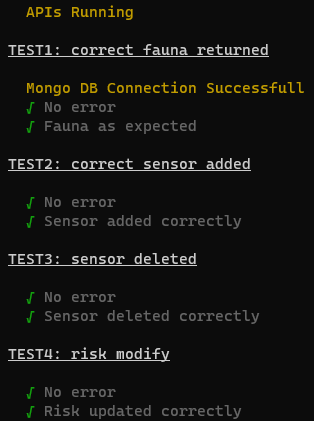
\includegraphics[scale=0.7]{Img/testing_result.png}
    \caption{Esito del testing}
\end{figure}